% !TEX root = ../thesis_main.tex
\chapter{Coherent Processes of Single-Wall Carbon Nanotubes}

\section{Introduction}
Coherent process occurs only during the presence of optical pump pulse. Often introduce so-called photon dressed states.

\section{Experimental Results}

\subsection{Optical Stark Effect}

Depends on pump intensity and detuning of pump with respect to photon energy of resonance. Observed in many different systems such as atoms, quantum dots, etc. Leads to a shift in the energy resonance.
\begin{figure}[H]
	\centering
	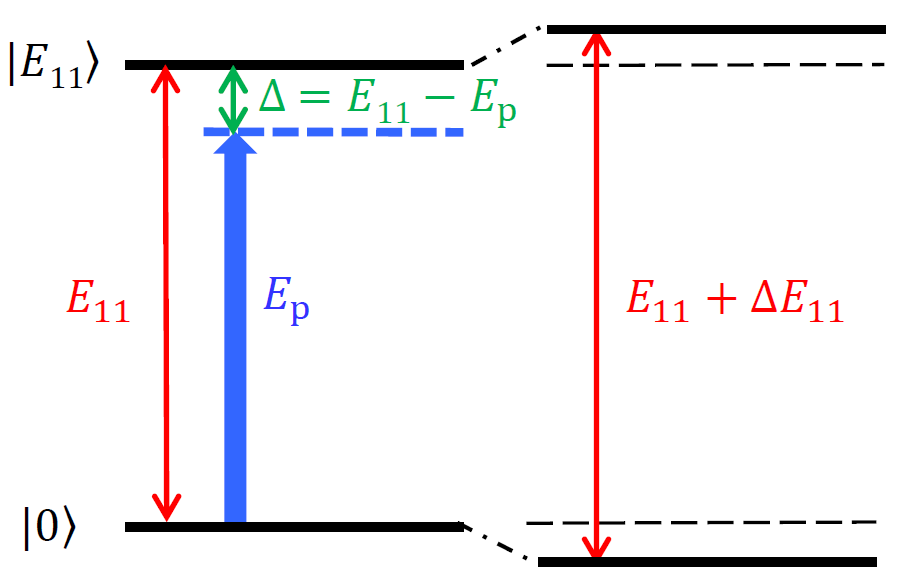
\includegraphics[scale=0.5]{images/chapter_coherent/kankan_stark_effect.png}
	\caption{Schematic Diagram of dressed states. Reproduced from Ref. .}
\end{figure}

Magnitude of the blueshift $\Delta E_{11}$ determined via the expression
\begin{equation}
		\Delta E_{11} = \sqrt{(\hbar \Omega_R)^2 + \Delta^2} - \Delta
\end{equation}

Under the condition that the detuning $\Delta \hbar \Omega_R\gg $, it can be shown that $\Delta E_{11} \propto I_p$ where $I_p$ represents the pump intensity \cite{mack}.
\subsection{Rabi Splitting}

Unusual because this is a Rabi splitting of exciton states

\begin{figure}[H]
	\centering
	\includegraphics{example-image-a}
	\caption{Schematic Diagram of dressed states. }
\end{figure}

\section{Data Analysis}

\section{Discussion}

Theory here provided by Weiwei Jiang and Prof. Mackillo Kira of the University of Michigan \cite{mack2019}.

\section{Conclusions}
